所有LLVM项目都遵循相同的目录结构。为了理解这个,让我们比较一下LLVM和GCC,即GNU编译器集合。几十年来,GCC几乎为您能想到的每一个系统都提供了成熟的编译器。但是,除了编译器,没有任何工具可以用这些代码,原因是它不为重用而设计。而LLVM截然不同。\par

每个功能都有明确的API定义,并放在自己的库中。clang项目有一个库,可以将C/C++源文件写入令牌流。解析器库将该令牌流转换为抽象语法树(由库支持)。语义分析、代码生成,甚至编译器驱动程序都作为库提供。众所周知的clang工具,只是一个链接到这些库的应用程序。\par

这样做的好处是显而易见的:当想要构建一个需要C++文件抽象语法树(AST)的工具时,您可以重用这些库的功能来构建AST。不需要语义分析和代码生成,也不需要链接这些库。所有LLVM项目都遵循这个原则,包括核心库!\par

每个项目都有类似的组织。因为CMake用于生成构建文件,所以每个项目都有一个CMakeLists.txt来描述项目的构建。如果需要额外的CMake模块或支持文件,可以将它们存储在cmake子目录中,而现成的模块则放在cmake/modules中。\par

库和工具大多是用C++编写的。源文件放在lib目录下,头文件放在include目录下。因为一个项目通常由几个库组成,所以lib目录中有每个库的目录。如果有必要,还会重复。例如,在llvm/lib目录中有Target目录,该目录包含特定于目标的更加底层的操作。除了一些源文件外,每个目标还有子目录,这些子目录会再次编译成库。每个目录都有一个CMakeLists.txt文件,该文件描述了如何构建库以及哪些子目录还包含源代码。\par

include目录有一个额外的级别。为了使包含文件的名称唯一,路径名包含项目名称,它是include下的第一个子目录。只有在这个文件夹中,lib目录的结构才会重复。\par

应用程序的源码位于tools和utils目录中。utils目录中是在编译或测试期间使用的内部应用程序。它们通常不是用户安装的一部分,tools目录包含用于最终用户的应用程序。这两个目录中,每个应用程序都有自己的子目录。与lib目录一样,每个包含source的子目录都有一个CMakeLists.txt文件。\par

编译器必须正确的生成代码,这需要通过一个好的测试套件来实现。unittest目录包含使用Google Test框架的单元测试。这主要用于单个函数和无法通过其他方式测试的独立功能。test目录中是LIT测试,这些测试使用llvm-lit实用程序执行测试。llvm-lit扫描文件中的shell命令并执行它们。该文件包含用作测试输入的源代码,例如:LLVM IR。文件中嵌入编译命令,由llvm-lit执行。然后,在FileCheck实用工具的帮助下,验证该步骤的输出。这个程序从一个文件中读取检查语句,并将它们与另一个文件进行匹配。LIT测试本身位于test目录下的子目录中,对于lib的目录结构的遵循不是很严格。\par

文档(通常是reStructuredText)放在docs目录中。如果项目提供了示例,则位于examples目录中。\par

根据项目的需要,还可以有其他目录。值得注意的是,一些提供运行时库的项目将源代码放在src目录中,并使用lib目录作为库导出定义。compiler-rt和libclc项目包含与体系结构相关的代码。它总是放在以目标体系结构命名的子目录中(例如,i386或ptx)。\par

总之,提供样例库并具有驱动工具项目的总体结构如下所示:\par

\hspace*{\fill} \par %插入空行
\begin{center}
	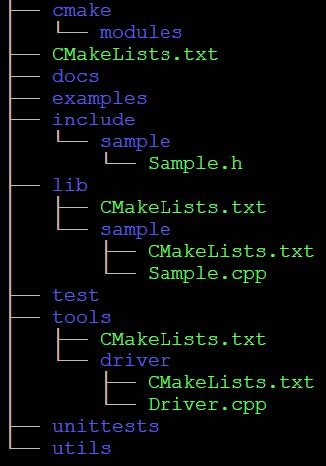
\includegraphics{content/1/chapter2/images/1.jpg}\\
	图2.1 – 项目的目录结构
\end{center}

我们自己的项目也将遵循这个结构。\par









